\chapter{Details}

Inclua aqui informações que não sejam tão relevantes para o entendimento do projeto mas que ainda sejam importantes para documentá-lo. 


put here the stability difficult about doing experiments

- syringe pump inclined
- pumping liquid to avoid bubbles
- mechanical noise in the pumping machine
- external electrical noise collected by antennas or connections

Foto e detalhes dos instrumentos

\begin{figure}[H]
    \centering
    \resizebox{150mm}{!}{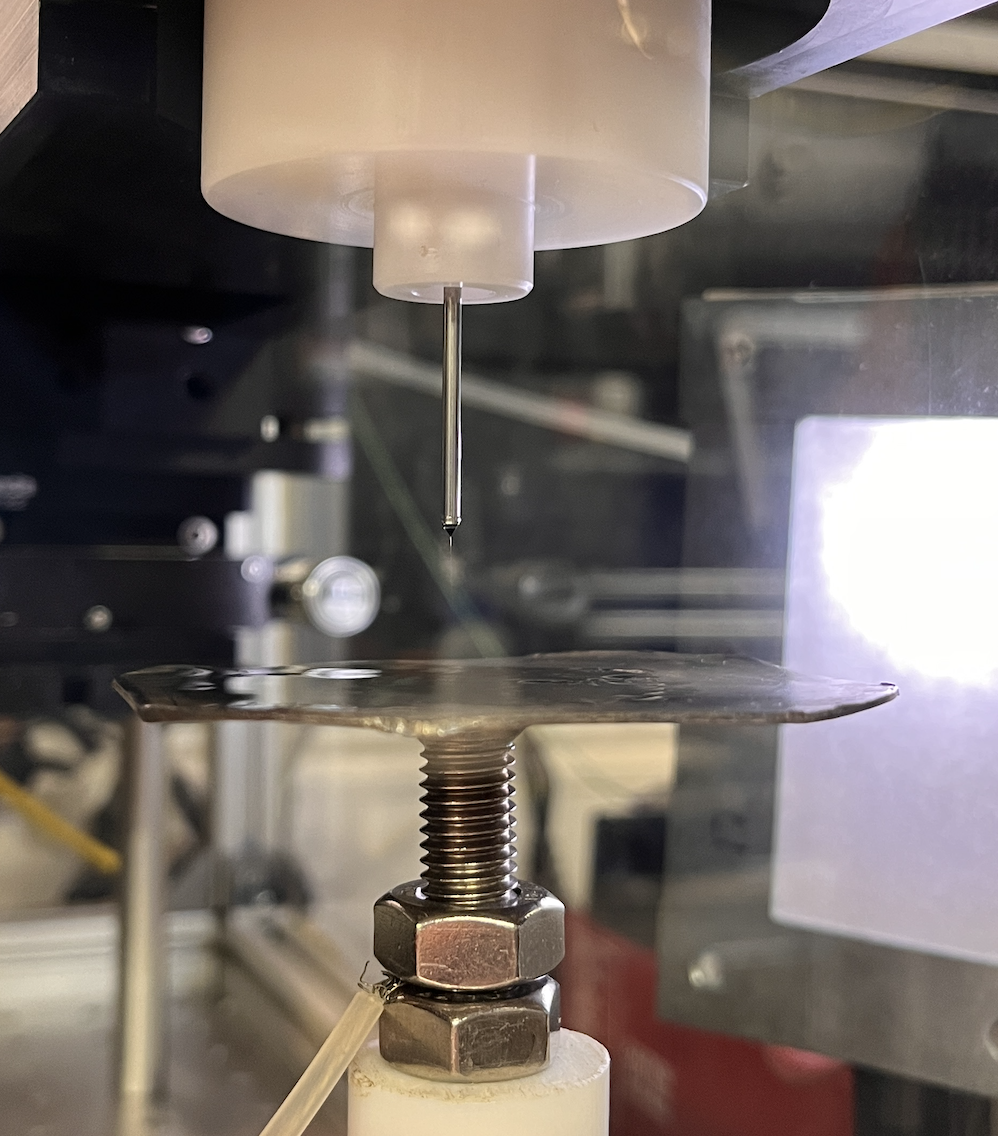
\includegraphics{Figuras/naked_eyes.png}}
    \caption{EHDA physical concept }
\end{figure}




\begin{figure}[H]
  \centering
  \resizebox{150mm}{!}{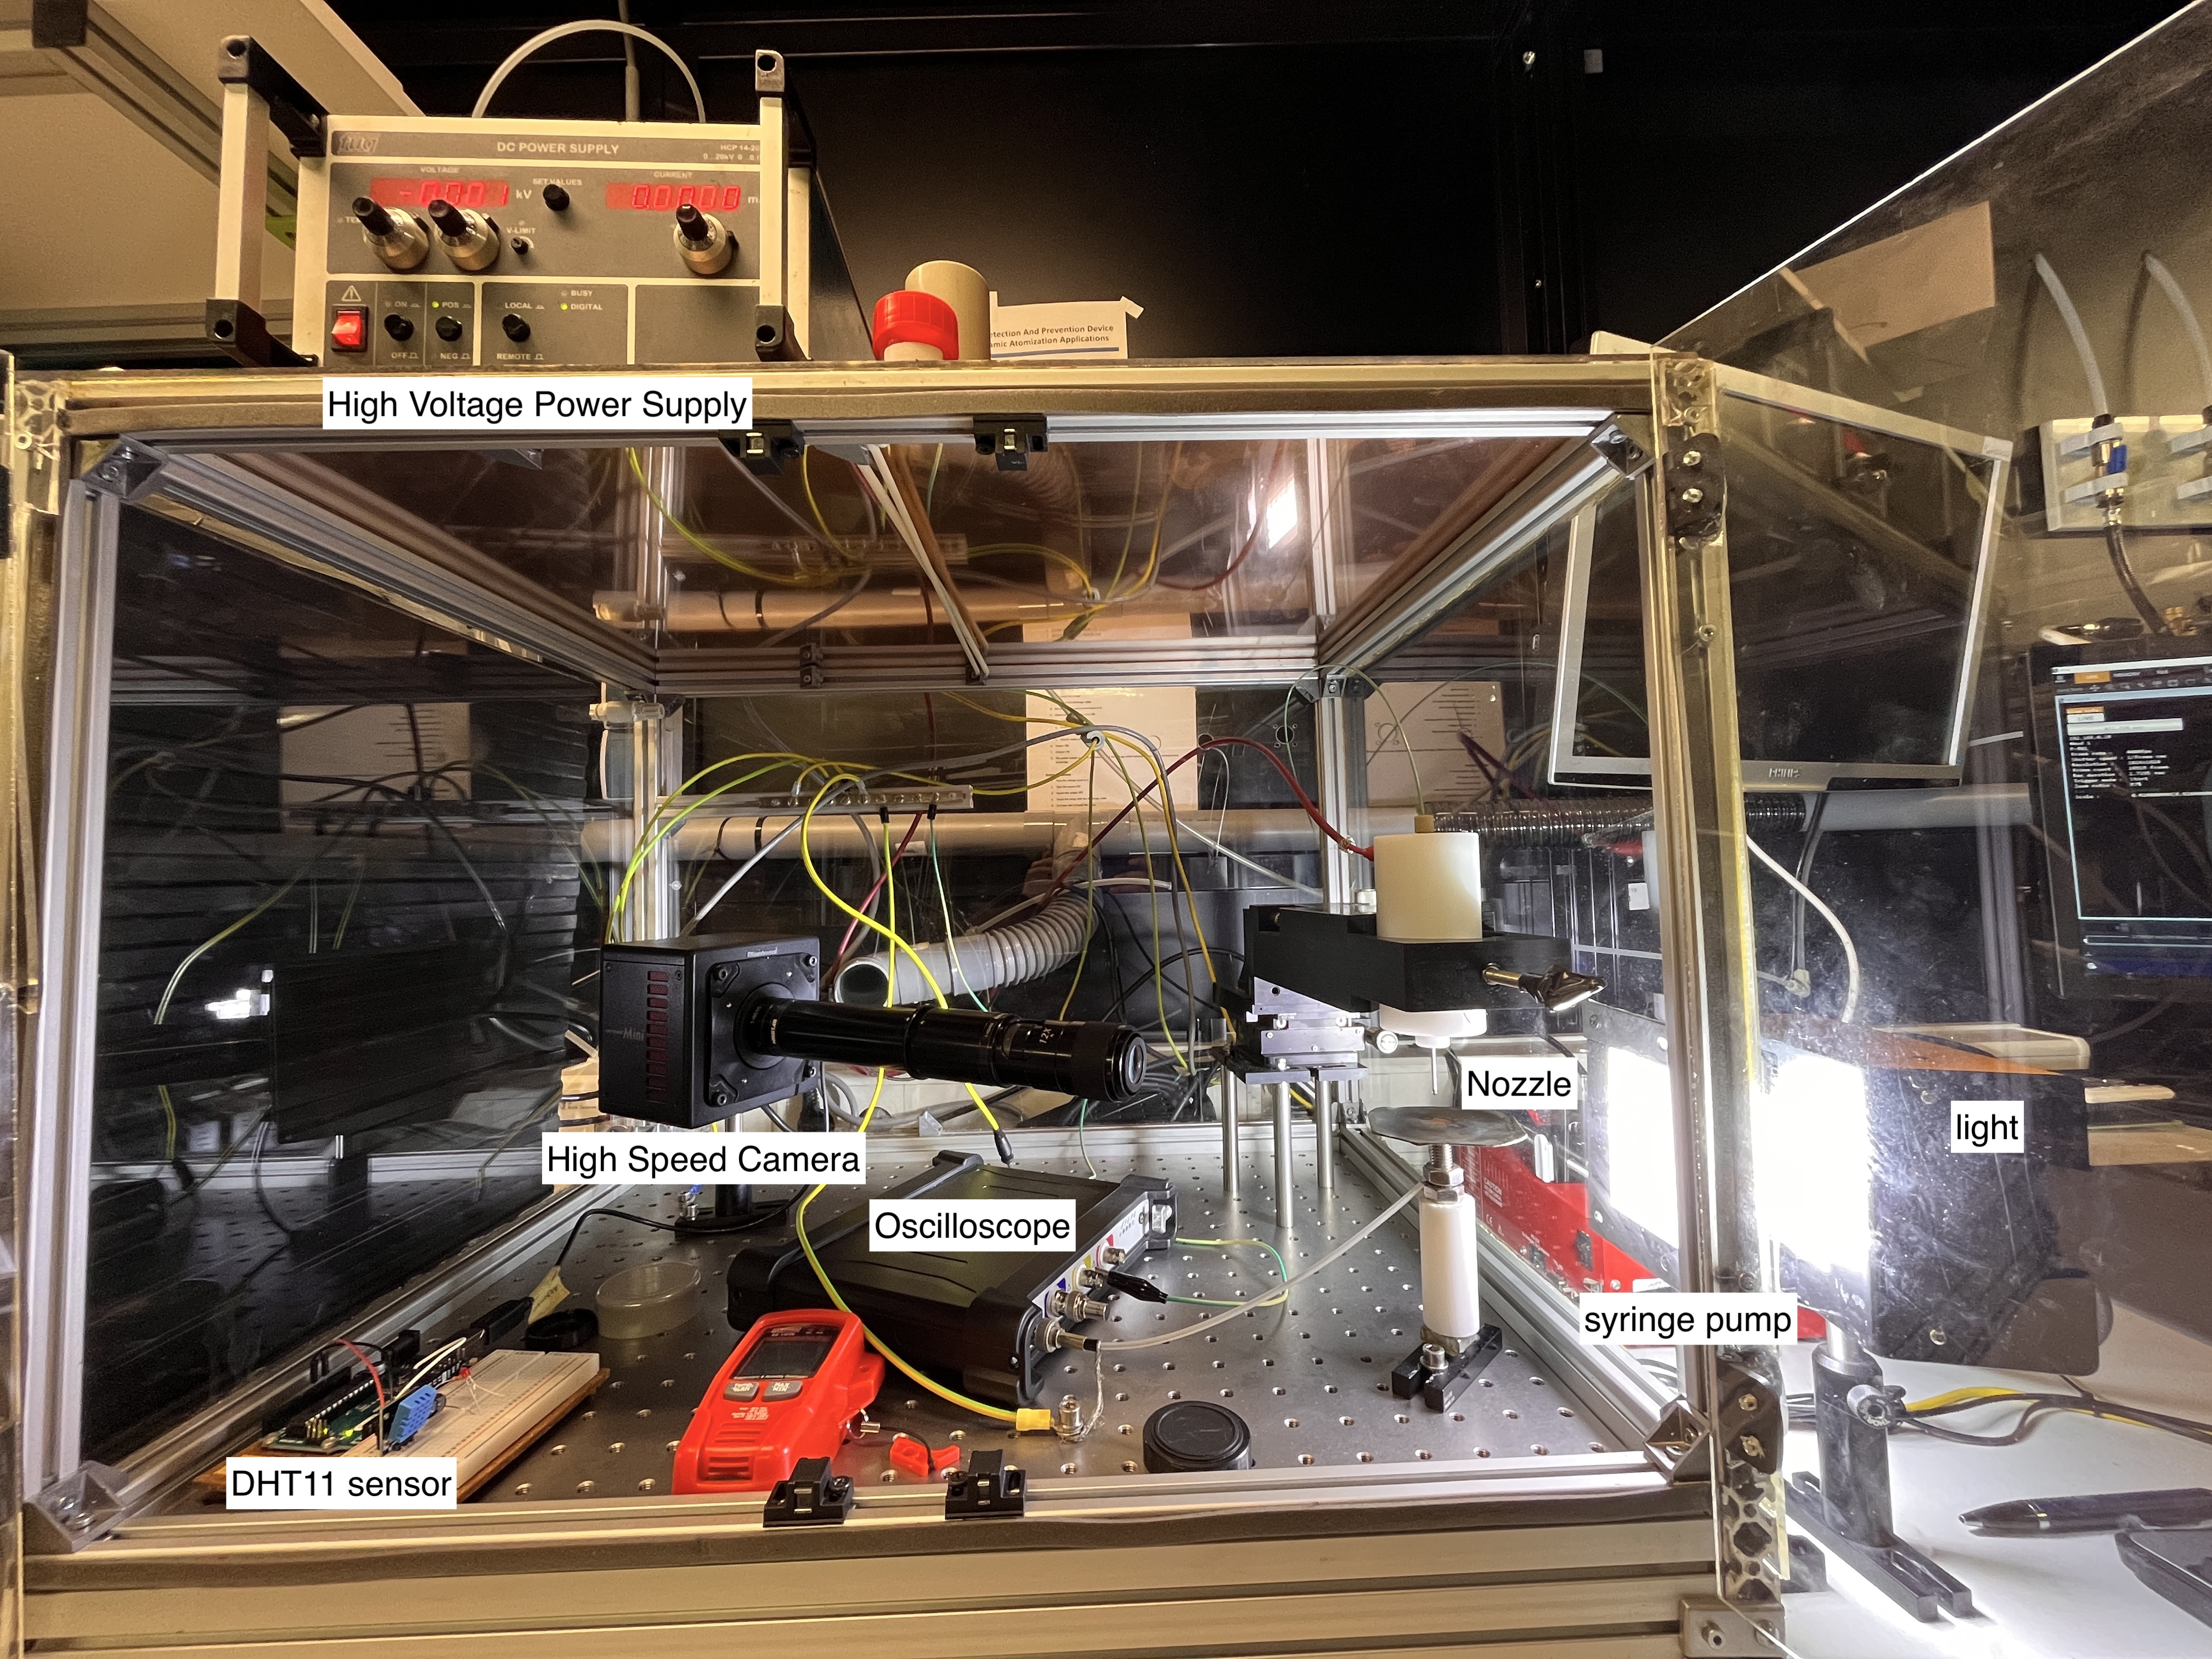
\includegraphics{Figuras/setup_pic.jpg}}
  \caption{EHDA automation system setup}
  \label{fig:setup_pic}
\end{figure}


\section{Setup Validation}
\label{sec:setup_validation}


Initial tests were made to verify the setup assembly and the automation routine integration. In this step I could understand in practice how electrospray works.
It was concluded that factors like geometry, polarity, material properties and occurring discharges are reflected in the system current.
Also, liquid properties such as surface tension, dielectric constant, viscosity, density, electrical conductivity and vacuum permittivity. 
 And also physical variables such as flow rate, system impedance, system temperature, system humidity, nozzle to plate distance, nozzle dimensions and applied voltage.


 About the setup, integrate was changed the liquid, nozzle diameter and distance to the plate in order to
make the experiment the most stable and easy to reach cone-jet mode as possible. For example, while doing experiments we discovered that the frequency of the pump machine internal motors was creating an interference in the flowrate. Therefore compromising the stabilization in cone jet mode. A solution for that was to increasethe flowrate wich smooths this pumping noise. For that was also necessary to increase the nozzle diameter to balance with all other variables from the experiment.
